\section{向量量化}
\label{sec:quant-vector}

传感器常常连续读数，相邻两次读数彼此接近。若把每个读数单独量化，量化器看不到这种联系。把两个读数合成一个二维向量，再整体选择重构点，能否在相同的每分量比特数下做得更好？这一节说明答案是肯定的，并说明好处来自哪里、代价在哪里。

\paragraph{逐分量码本与联合码本}
对$d$维读数$\bm{X}=(X_1,\dots,X_d)$，最直接的做法是给每个分量配一个标量量化器，各分量独立编码。若第$i$个分量用$N_i$个点，合起来的重构点是各分量重构值的全部组合，共$N=N_1\cdots N_d$个，区域是坐标轴方向的长方体。这样的量化器称为\term{乘积量化器}（product quantizer），它的码本称为逐分量码本。

更一般的做法是直接在$\mathbb{R}^{d}$中选$N$个点$\bm{c}_1,\dots,\bm{c}_N$作为码本，区域不必是长方体。这就是第~\ref{sec:quant-model}节定义中的$d$维量化器，称为\term{向量量化}（vector quantization），它的码本称为联合码本。乘积量化器是它的特例，所以在相同点数下，最好的联合码本不会比最好的逐分量码本差。按式~\eqref{eq:quant-rate-per-component}，两者每分量的比特数都是$\frac1d\log_2N$。

\paragraph{两条条件的推广}
平方误差取$\lVert\bm{x}-\hat{\bm{x}}\rVert_2^{2}$。第~\ref{sec:quant-nonuniform}节的两个引理在$d$维中照样成立，证明只需把乘积换成内积。

对质心条件，设区域$S$的概率$p>0$，条件均值$\bm{m}=\mathbb{E}[\bm{X}\mid\bm{X}\in S]$。展开平方范数，
\[
 \lVert\bm{X}-\bm{c}\rVert_2^{2}=\lVert\bm{X}-\bm{m}\rVert_2^{2}+2\langle\bm{X}-\bm{m},\bm{m}-\bm{c}\rangle+\lVert\bm{m}-\bm{c}\rVert_2^{2} .
\]
交叉项乘$\mathbf{1}_{\{\bm{X}\in S\}}$后期望为零，于是
\begin{equation}
 \mathbb{E}\bigl[\lVert\bm{X}-\bm{c}\rVert_2^{2}\mathbf{1}_{\{\bm{X}\in S\}}\bigr]=\mathbb{E}\bigl[\lVert\bm{X}-\bm{m}\rVert_2^{2}\mathbf{1}_{\{\bm{X}\in S\}}\bigr]+p\lVert\bm{m}-\bm{c}\rVert_2^{2} ,
 \label{eq:quant-vector-parallel-axis}
\end{equation}
最好的重构点仍是区域的质心。最近邻条件的证明与维数无关，逐点取最近的重构点即可。

最近邻规则下的区域有明确的几何形状。$\bm{x}$离$\bm{c}_j$不比离$\bm{c}_k$远，即
\[
 \lVert\bm{x}-\bm{c}_j\rVert_2^{2}\leq\lVert\bm{x}-\bm{c}_k\rVert_2^{2} .
\]
展开两边，$\lVert\bm{x}\rVert_2^{2}$相消，条件化为
\[
 2\langle\bm{x},\bm{c}_k-\bm{c}_j\rangle\leq\lVert\bm{c}_k\rVert_2^{2}-\lVert\bm{c}_j\rVert_2^{2} .
\]
这是以$\bm{c}_j$与$\bm{c}_k$连线的垂直平分面为边界的半空间。对所有$k\neq j$取交集，得到
\begin{equation}
 V_j=\bigl\{\bm{x}\in\mathbb{R}^{d}:\ \lVert\bm{x}-\bm{c}_j\rVert_2\leq\lVert\bm{x}-\bm{c}_k\rVert_2,\ k=1,\dots,N\bigr\} ,
 \label{eq:quant-voronoi}
\end{equation}
称为$\bm{c}_j$的\term{Voronoi区域}（Voronoi region）。它是有限个半空间的交，因而是凸多面体（可以无界）。各$V_j$只在边界上重叠，边界属于哪一个仍按编号约定；一维时它们就是以中点为端点的区间。

\paragraph{广义Lloyd算法}
于是标量的交替改进可以原样搬过来：固定码本，按式~\eqref{eq:quant-voronoi}把读数分给最近的码字；固定区域，把每个码字移到区域的质心。第~\ref{sec:quant-nonuniform}节的单调性论证逐字适用，平均失真单调不增。这一推广称为\term{广义Lloyd算法}（generalized Lloyd algorithm）。

二维以上的区域是多边形或多面体，质心一般没有显式公式。实际计算时，常用从源分布模拟出的大量向量的平均代替期望：区域的质心换成落在区域中的模拟向量的平均，平均失真换成模拟向量的平均误差。这样得到的是对期望的近似，其误差由第~\ref{chap:monte-carlo-integration-error}章的方法估计；若这些向量不是模拟出来的，而是观测到的数据，从数据估计量化器就属于统计推断的问题，由卷八处理。

\paragraph{相关结构的利用}
先看一个可以手算的例子。读数$\bm{X}=(X_1,X_2)$在两个单位正方形的并集
\[
 A=[0,1]^{2}\cup[1,2]^{2}
\]
上均匀分布，两个正方形各占概率$\tfrac12$。两个分量高度相关：$X_1$小时$X_2$也小。每个分量允许1 bit，即$N=4$。

先用逐分量码本。$X_1$的分布是$[0,1]$与$[1,2]$上各一半的均匀分布，合起来是$[0,2]$上的均匀分布，$X_2$也一样。每个分量最好的两点量化器取区间中点$0.5$与$1.5$，每分量误差为
\[
 \mathbb{E}\bigl[(X_1-Q_1(X_1))^{2}\bigr]=\frac{1^{2}}{12}=\frac{1}{12},
\]
每个向量的平方误差为$\tfrac16$。四个组合点中，$(0.5,1.5)$与$(1.5,0.5)$落在两个空白方块里，它们的区域概率为零，从不被使用。图~\ref{fig:quant-two-squares}左图画出了这种浪费。

\begin{BookInlineFigure}
 \centering
 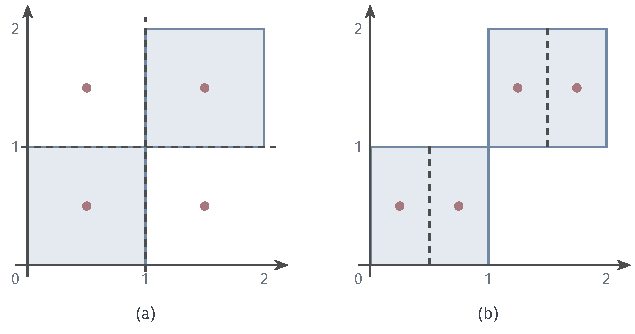
\includegraphics[width=107.5mm]{figures/07-probability/05-source-coding/tikz/quant-two-squares/figure.pdf}
 \caption{在两个单位正方形（浅蓝）上均匀分布的二维读数，用4个点量化。(a) 逐分量码本：每个分量取$0.5$与$1.5$，红点是全部4个组合，虚线是区域边界；两个点落在空白处，从不使用，每个向量的平方误差为$1/6$。(b) 联合码本：每个正方形沿竖直中线一分为二，各放一个质心，平方误差为$5/48$。}
 \label{fig:quant-two-squares}
\end{BookInlineFigure}

若对这个逐分量码本运行广义Lloyd算法，第一轮最近邻分配就会使两个空白方块中的码字分不到任何读数，出现第~\ref{sec:quant-nonuniform}节所说的空区域。按“挪到误差最大的区域并一分为二”的处理，每个被使用的码字区域分出一半给空闲码字，得到右图的联合码本：
\[
 (0.25,0.5),\quad(0.75,0.5),\quad(1.25,1.5),\quad(1.75,1.5) .
\]
每个区域是$\tfrac12\times1$的长方形，读数在其中均匀分布。由式~\eqref{eq:quant-vector-parallel-axis}，以质心为重构点时，误差就是两个坐标方向的方差之和，
\[
 \frac{(1/2)^{2}}{12}+\frac{1^{2}}{12}=\frac{1}{48}+\frac{4}{48}=\frac{5}{48} .
\]
这组码本满足两条条件：每个码字是区域质心，区域也正是最近邻区域。联合码本把每个向量的平方误差从$\tfrac{8}{48}$降到$\tfrac{5}{48}$，减少$37.5\%$，而每分量仍是1 bit。好处来自把四个点全部放在读数真正出现的地方。

图~\ref{fig:quant-gauss-vq}对连续分布做同样的比较。读数是相关系数$0.9$、方差为$1$的二维高斯向量，$N=16$，每分量2 bit。左图是两个4点Lloyd--Max标量量化器的乘积，每分量误差是标量值$0.1175$。十六个长方形中只有十个的概率超过千分之一，其余几乎不用。右图是从左图码本出发、在$2\times10^{5}$个模拟向量上运行广义Lloyd算法得到的联合码本：码字沿对角线排成一串，区域是与对角线垂直的长条。在另外$2\times10^{5}$个独立模拟向量上计算，每分量误差约为$0.0442$，不到逐分量码本的四成。

\begin{BookInlineFigure}
 \centering
 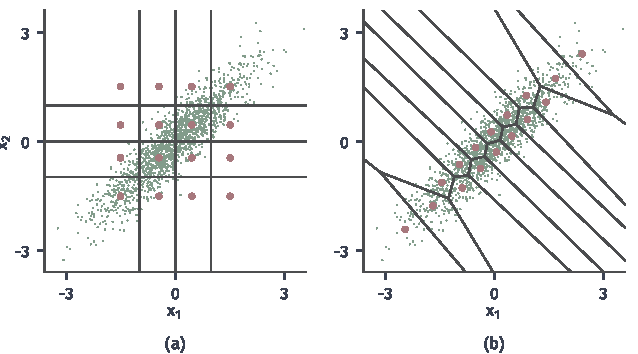
\includegraphics[width=108mm]{figures/07-probability/05-source-coding/matplotlib/quant-gauss-vq/figure.pdf}
 \caption{相关系数$0.9$的二维标准高斯读数，16个码字。绿点为1500个模拟读数，红点为码字，灰线为区域边界。(a) 逐分量4点Lloyd--Max码本，每分量误差$0.1175$。(b) 广义Lloyd算法得到的联合码本（$2\times10^{5}$个训练向量，种子1），区域为Voronoi区域；在独立的$2\times10^{5}$个向量（种子2）上每分量误差约为$0.0442$。}
 \label{fig:quant-gauss-vq}
\end{BookInlineFigure}

\paragraph{区域形状的利用}
即使分量相互独立，联合码本仍有一点好处，来自区域的形状。设读数在一个区域内近似均匀分布，区域面积为$V$，重构点在区域的质心。为了比较形状而不受大小影响，把每分量的平方误差除以$V^{2/d}$，得到无量纲的\term{归一化二阶矩}（normalized second moment）
\begin{equation}
 G=\frac{1}{d}\,\frac{1}{V^{1+2/d}}\int_{\text{区域}}\lVert\bm{x}-\bm{c}\rVert_2^{2}\,\mathrm{d}\bm{x} ,
 \label{eq:quant-normalized-moment}
\end{equation}
$G$越小，同样面积的区域给出的误差越小。逐分量量化在独立同分布的分量上产生正方形区域，联合码本可以用其他形状铺满平面。

单位正方形以中心为重构点时，两个方向各贡献$\tfrac1{12}$，所以$G=\tfrac1{12}\approx0.0833$。正六边形可以用平行轴恒等式~\eqref{eq:quant-vector-parallel-axis}计算。把边长为$a$的正六边形分成六个边长为$a$的正三角形，每个三角形的面积为$A_{\triangle}=\frac{\sqrt3}{4}a^{2}$，直接积分可得它绕自身质心的二阶矩是$A_{\triangle}a^{2}/12$。三角形的质心离六边形中心$a/\sqrt3$，由式~\eqref{eq:quant-vector-parallel-axis}，绕六边形中心的二阶矩为
\[
 A_{\triangle}\Bigl(\frac{a^{2}}{12}+\frac{a^{2}}{3}\Bigr)=\frac{5}{12}A_{\triangle}a^{2} .
\]
六个三角形合起来，面积为$6A_{\triangle}$，二阶矩为$6\cdot\frac{5}{12}A_{\triangle}a^{2}$。取面积为$1$，即$a^{2}=\frac{2}{3\sqrt3}$，代入式~\eqref{eq:quant-normalized-moment}，
\[
 G=\frac12\cdot\frac{5}{12}a^{2}=\frac{5}{36\sqrt3}\approx0.0802 .
\]

\begin{BookInlineFigure}
 \centering
 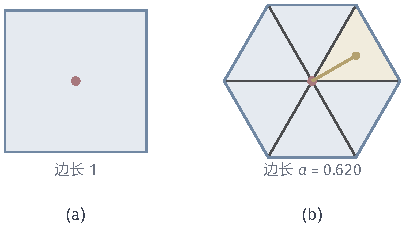
\includegraphics[width=68.6mm]{figures/07-probability/05-source-coding/tikz/quant-cell-shapes/figure.pdf}
 \caption{面积同为$1$的两种区域，红点为重构点。(a) 正方形，$G=1/12\approx0.0833$。(b) 正六边形分成六个正三角形；黄色三角形的质心（黄点）离中心$a/\sqrt3$，由平行轴恒等式求得$G=5/(36\sqrt3)\approx0.0802$。}
 \label{fig:quant-cell-shapes}
\end{BookInlineFigure}

图~\ref{fig:quant-cell-shapes}比较了这两种形状。六边形比正方形更接近圆，离重构点远的角少，在相同面积下误差约小$3.8\%$。这个收益只在区域很多、边界效应可以忽略时才显现，而且只有联合码本才能取得，因为逐分量量化的区域永远是长方体。与相关结构带来的收益相比，形状收益不大；但它说明即使分量独立，逐个读数量化也不是最好的做法。

\paragraph{存储、搜索与局部最优的代价}
联合码本的收益需要付出代价。固定每分量$R$个比特，码字个数为
\begin{equation}
 N=2^{dR} ,
 \label{eq:quant-codebook-size}
\end{equation}
随维数$d$指数增长。表~\ref{tab:quant-vq-cost}列出几种情形：存储码本需要$Nd$个实数，对每个读数做穷举最近邻搜索需要计算$N$个距离，约$Nd$次乘法。逐分量码本只需存储$d$个标量量化器，共$d2^{R}$个数，编码时各分量独立查找。

\begin{BookInlineTable}
 \centering
 \begin{tabular}{rrrrr}
  \toprule
  $d$ & $R$ & $N=2^{dR}$ & 联合码本存储$Nd$ & 逐分量存储$d2^{R}$\\
  \midrule
  $2$ & $2$ & $16$ & $32$ & $8$\\
  $4$ & $2$ & $256$ & $1024$ & $16$\\
  $8$ & $2$ & $65536$ & $524288$ & $32$\\
  $16$ & $1$ & $65536$ & $1048576$ & $32$\\
  \bottomrule
 \end{tabular}
 \caption{每分量$R$ bit时联合码本与逐分量码本的规模。穷举搜索每个读数的乘法次数与联合码本存储量同阶。}
 \label{tab:quant-vq-cost}
\end{BookInlineTable}

设计码本也更困难。广义Lloyd算法每轮要对每个模拟向量计算$N$个距离，而且目标函数有许多局部最小值，结果依赖初值。图~\ref{fig:quant-vq-inits}在前面的相关高斯例子上，从十组随机初值出发各迭代四十轮：所有轨迹都降到逐分量码本的误差之下，最终的每分量误差分布在$0.0439$到$0.0455$之间，彼此相差约$4\%$。维数和码字更多时，这种差异通常更大。

\begin{BookInlineFigure}
 \centering
 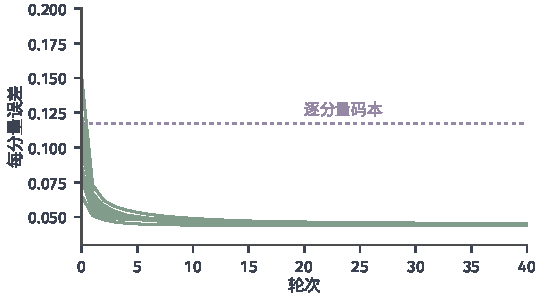
\includegraphics[width=92mm]{figures/07-probability/05-source-coding/matplotlib/quant-vq-inits/figure.pdf}
 \caption{相关系数$0.9$的二维高斯读数、16个码字时，广义Lloyd算法从十组初值出发的每分量误差（绿线，在$5\times10^{4}$个模拟向量上计算，种子1；初值为随机抽取的16个模拟向量，种子11至20）。紫色点线为逐分量4点Lloyd--Max码本的误差$0.1175$。各轨迹单调下降，但停在不同的值上。}
 \label{fig:quant-vq-inits}
\end{BookInlineFigure}

所以向量量化的维数是一种权衡：维数越高，越能利用相关结构和区域形状，码本存储、搜索和设计的代价也越高。实际系统常用有结构的码本（例如由格点构成的码本，或分级、分组的码本）来降低搜索代价，代价是放弃一部分失真上的收益。
